\section{Wdrożenie Systemu}
\label{sec:Wdrozenie_systemu}

Rozdział opisuje infrastrukturę, na której działa system, sposób jej konfiguracji oraz scenariusze użycia z perspektywy użytkownika.

\begin{figure}[H]
  \centering
  \includegraphics[width=\linewidth]{img/06_wdrozenie_systemu/C4Deployment.png}
  \caption{Diagram wdrożenia systemu --- konkretne zasoby AWS, adresy i porty}
  \label{fig:deployment-diagram}
\end{figure}

\subsection{Infrastruktura Terraform}

Infrastruktura AWS jest zdefiniowana jako kod przy użyciu Terraform \cite{hashicorp_terraform}. Definicje znajdują się w katalogu \texttt{devops/terraform/} i obejmują wszystkie zasoby potrzebne do działania projektu. Zastosowane podejście IaC (Infrastructure as Code) pozwala odtworzyć całe środowisko jedną komendą \texttt{terraform apply}, bez ręcznego klikania w konsoli AWS.

Pliki konfiguracyjne są podzielone według odpowiedzialności:
\begin{itemize}
  \item \texttt{main.tf} --- zasoby EC2, VPC, sieci,
  \item \texttt{s3.tf} --- zasobniki S3 i uprawnienia,
  \item \texttt{ecr.tf} --- rejestr obrazów Docker,
  \item \texttt{iam.tf} --- role i polityki IAM,
  \item \texttt{variables.tf} --- deklaracje zmiennych z wartościami domyślnymi,
  \item \texttt{terraform.tfvars} --- konkretne wartości zmiennych (region, typ instancji, IP operatora).
\end{itemize}

Tworzone zasoby:
\begin{itemize}
  \item \textbf{VPC i podsieć publiczna} --- prosta sieć z bezpośrednim dostępem do internetu przez Internet Gateway; eliminuje potrzebę NAT Gateway (oszczędność \textasciitilde\$32/miesiąc),
  \item \textbf{Security Group} --- reguły ruchu przychodzącego i wychodzącego opisane w sekcji~\ref{subsec:porty},
  \item \textbf{Instancja EC2} --- typ \texttt{t3.large} (8~GB RAM, 2~vCPU); konfigurowalny przez zmienną \texttt{instance\_type} w \texttt{terraform.tfvars},
  \item \textbf{Amazon S3} --- dwa zasobniki: \texttt{wms-dvc-data-*} dla danych treningowych DVC i \\\texttt{wms-mlflow-artifacts-*} dla artefaktów MLflow,
  \item \textbf{Amazon ECR} --- rejestr obrazów Docker dla API modelu,
  \item \textbf{IAM Role} --- rola instancji EC2 z uprawnieniami do odczytu i zapisu S3 oraz ECR; rola jest przypisywana do instancji, co eliminuje potrzebę przechowywania kluczy AWS na maszynie.
\end{itemize}

Infrastruktura uruchamiana jest jednorazowo poleceniem \texttt{terraform apply} (rys.~\ref{fig:terraform-apply}), nie tworzona od nowa przy każdym treningu. Zasoby statyczne (VPC, S3, ECR, IAM) istnieją przez cały czas życia projektu. Instancja EC2 jest natomiast zatrzymywana po każdym uruchomieniu pipeline'u i wznawiana tylko na czas treningu lub wdrożenia, co istotnie obniża koszty eksploatacji.
\begin{figure}[H]
  \centering
  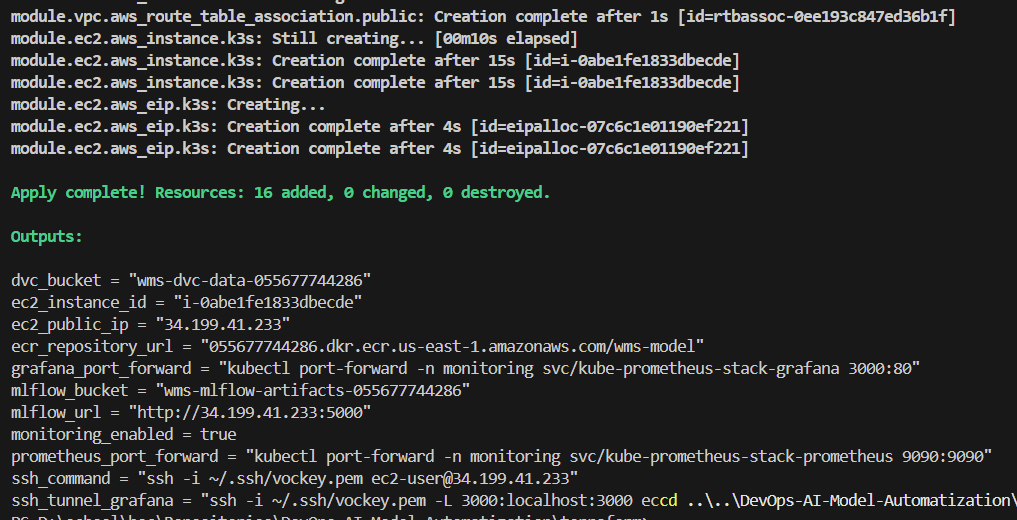
\includegraphics[width=\linewidth]{img/06_wdrozenie_systemu/terraform_apply.png}
  \caption{Wynik polecenia \texttt{terraform apply} --- lista 12 utworzonych zasobów AWS}
  \label{fig:terraform-apply}
\end{figure}

Rysunki~\ref{fig:aws-ec2} i~\ref{fig:aws-s3} przedstawiają odpowiednio instancję EC2 i zasobniki S3 w konsoli AWS.

\begin{figure}[H]
  \centering
  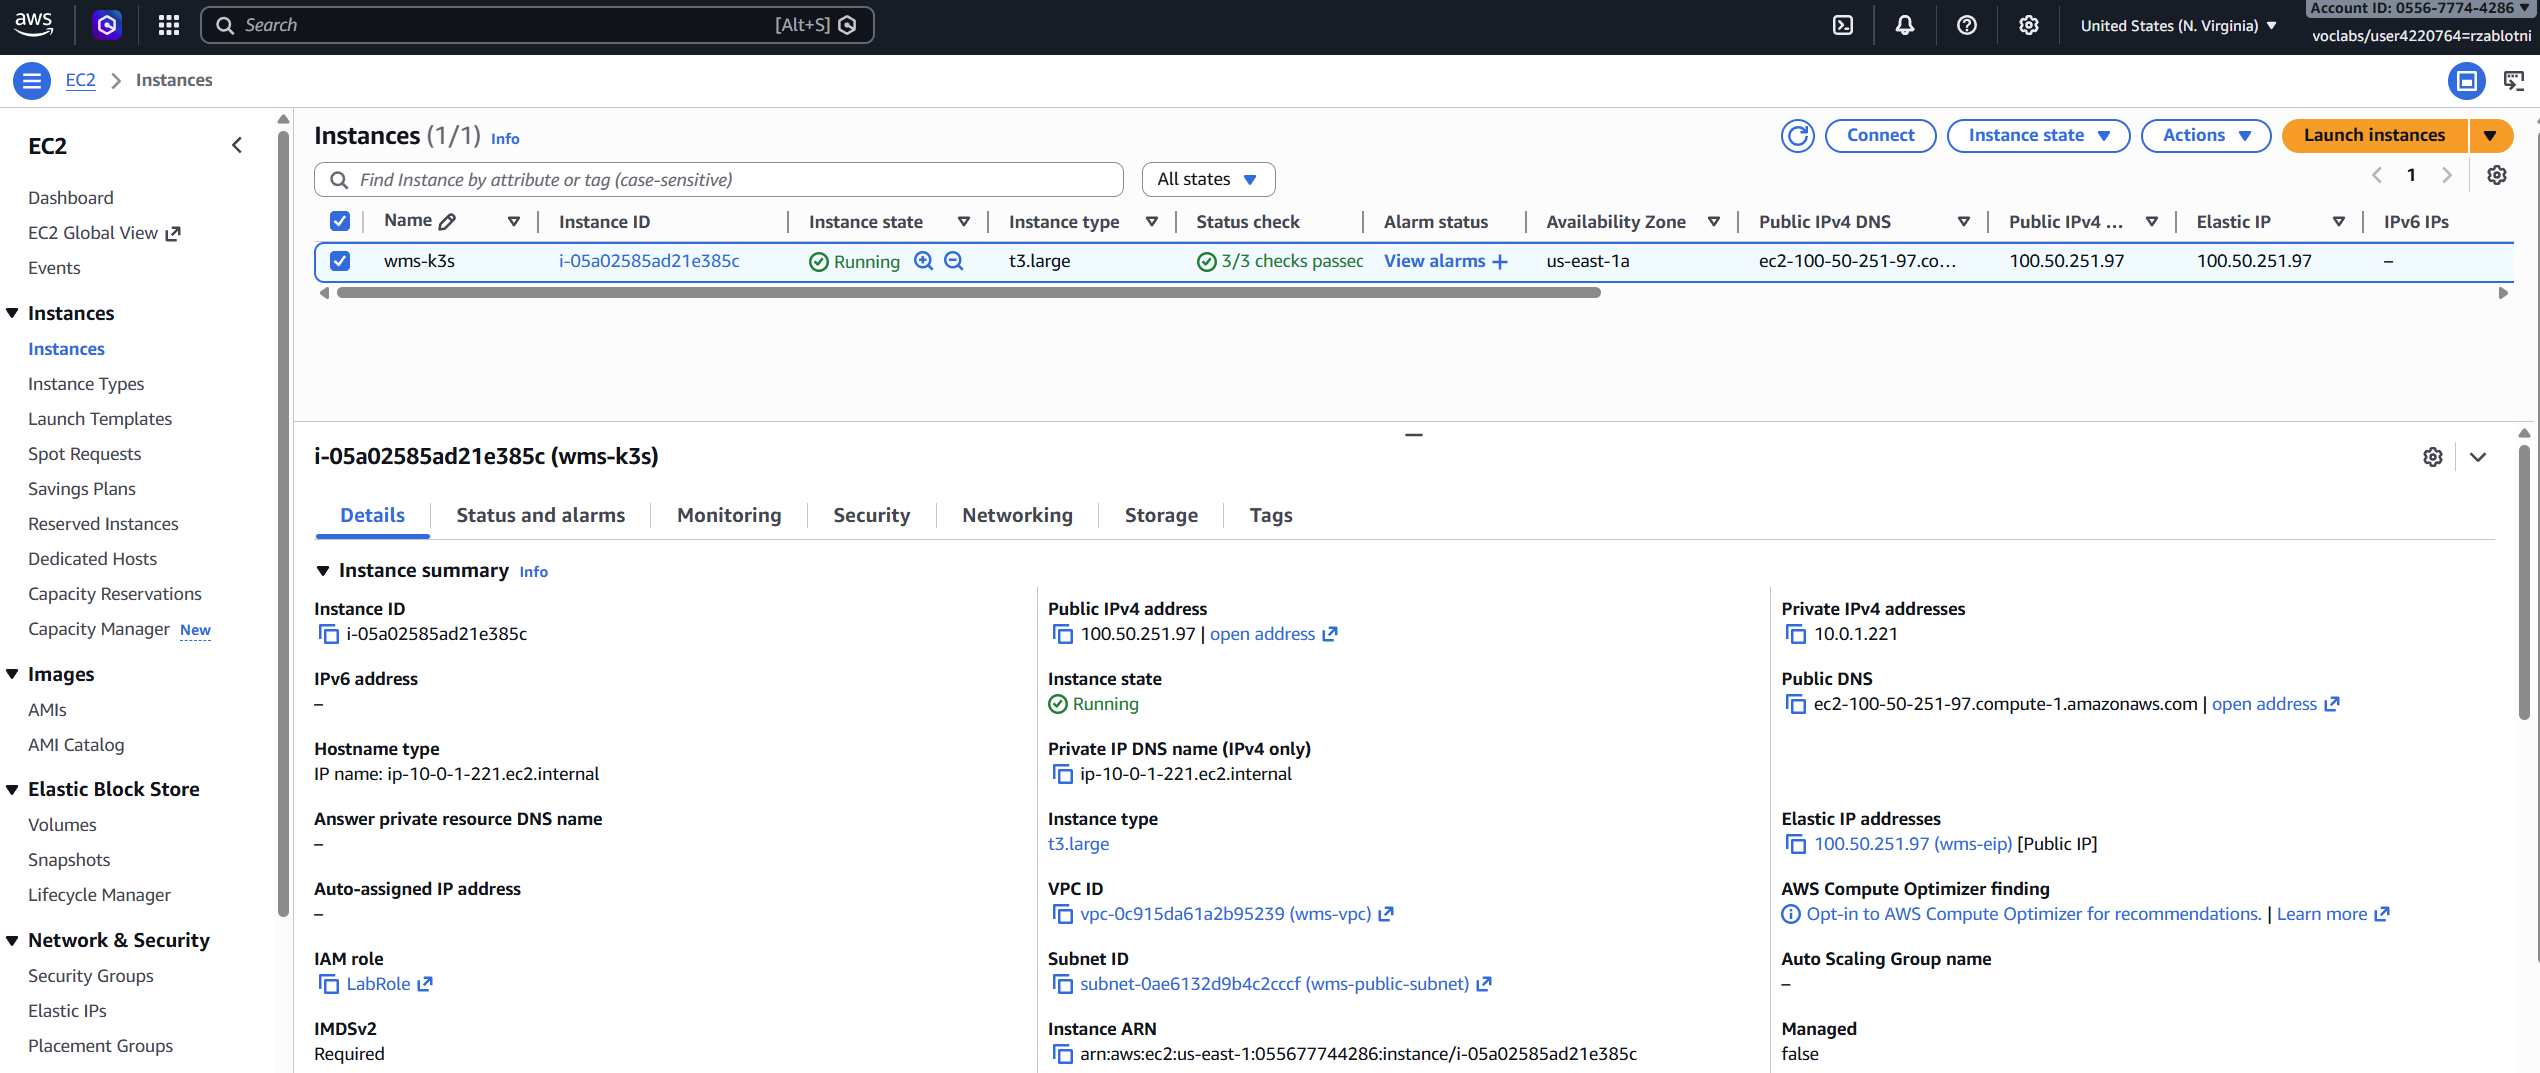
\includegraphics[width=\linewidth]{img/06_wdrozenie_systemu/aws_ec2_console.png}
  \caption{Instancja EC2 \texttt{wms-k3s} w konsoli AWS}
  \label{fig:aws-ec2}
\end{figure}
\vspace{-30pt}
\begin{figure}[H]
  \centering
  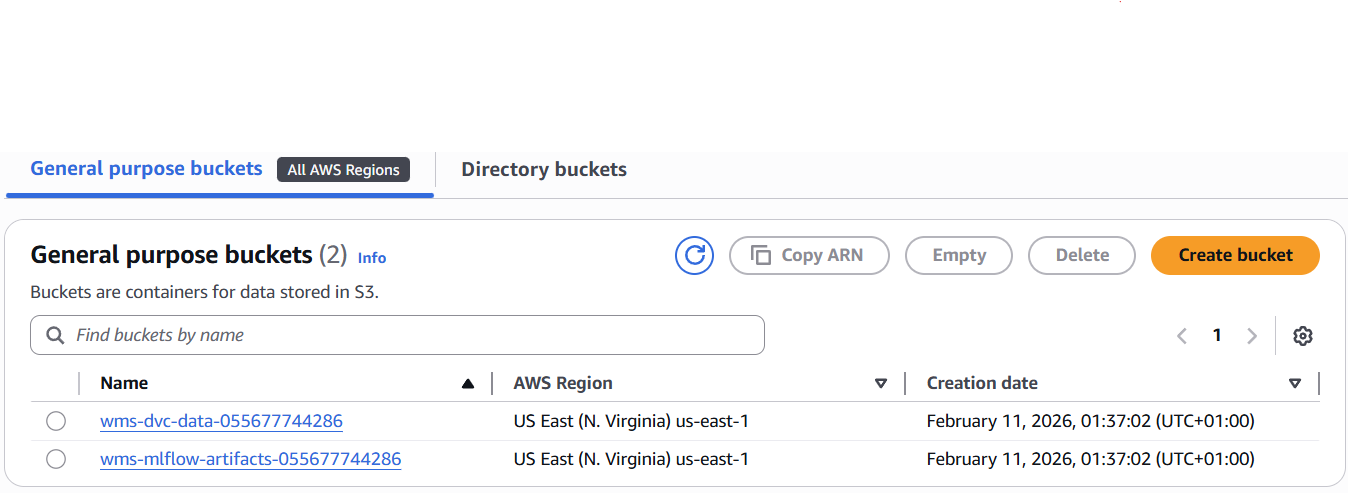
\includegraphics[width=\linewidth]{img/06_wdrozenie_systemu/aws_s3_buckets.png}
  \caption{Zasobniki S3: \texttt{wms-dvc-data-*} dla danych treningowych i \texttt{wms-mlflow-artifacts-*} dla artefaktów}
  \label{fig:aws-s3}
\end{figure}
\vspace{5pt}

\subsection{Konfiguracja EC2 i k3s}

Konfiguracja instancji EC2 odbywa się automatycznie przy pierwszym uruchomieniu za pomocą skryptu \texttt{user-data}. Skrypt jest szablonowany przez Terraform, który przy generowaniu pliku podstawiane są zmienne takie jak adres zasobnika S3 i region AWS, dzięki czemu nie ma żadnych wartości zakodowanych na stałe.

Kroki wykonywane przez \texttt{user-data}:
\begin{enumerate}
  \item Instalacja zależności systemowych: \texttt{dnf install -y git curl libicu}.
  \item Instalacja k3s --- uproszczonego Kubernetes \cite{k3s_docs}.
  \item Instalacja MLflow i boto3: \texttt{pip3 install --ignore-installed mlflow boto3}.
  \item Konfiguracja MLflow jako usługi systemd:
\begin{verbatim}
[Service]
ExecStart=mlflow server \
  --host 0.0.0.0 --port 5000 \
  --default-artifact-root s3://${mlflow_bucket}/
\end{verbatim}
  \item Instalacja GitHub Actions runnera jako usługi systemd.
\end{enumerate}

Instancja korzysta z Amazon Linux 2023, który oferuje nowszy OpenSSL 3.0 i wsparcie producenta do 2028 roku. Po zakończeniu \texttt{user-data} instancja jest gotowa do przyjęcia zadań z GitHub Actions bez dalszej konfiguracji ręcznej.

\textbf{Architektura k3s.} K3s to uproszczona dystrybucja Kubernetes zawarta w pojedynczym pliku binarnym. W porównaniu do pełnego Kubernetes zastępuje etcd bazą SQLite, usuwa przestarzałe sterowniki i wbudowuje podstawowe komponenty sieciowe. Dzięki temu działa na instancji \texttt{t3.large} (8~GB RAM) ze znaczącym zapasem zasobów dla poda z modelem; pełne Kubernetes samo w sobie wymagałoby podobnej ilości RAM.

W projekcie użyty jest klaster jednorazłowy (single-node): jeden węzeł pełni jednocześnie rolę control plane i workera. Taka architektura jest wystarczająca dla jednej działającej aplikacji i eliminuje koszty dodatkowych instancji EC2. Wysoka dostępność (HA) nie była wymaganiem. System jest przeznaczony do demonstracji i testowania, nie do środowiska produkcyjnego.

\textbf{Strategia aktualizacji.} Dla Deploymentu zastosowano domyślną strategię \texttt{RollingUpdate}: k3s najpierw uruchamia nowy pod, a dopiero po jego gotowości usuwa stary. Oznacza to zerowy przestój (zero-downtime deployment) przy aktualizacji modelu. Działa to jednak tylko wtedy, gdy instancja EC2 jest uruchomiona. W przeciwnym wypadku klaster jest niedostępny.

\textbf{Rollbacki i wersjonowanie.} Rollbacki na poziomie Kubernetes nie są rozbudowane celowo. Mechanizmem wersjonowania modeli jest MLflow, gdzie każda wersja modelu jest zarejestrowana w rejestrze MLflow ze swoimi metrykami. Rollback polega na przestawieniu stadium modelu w MLflow z \texttt{Production} na poprzednią wersję i ponownym uruchomieniu \texttt{deploy-model.yaml}. Helm zachowuje historię ostatnich wdrożeń (\texttt{helm history wms-api}), co umożliwia też cofnięcie konfiguracji Kubernetes bez ponownego treningu.

Rysunek~\ref{fig:systemctl-status} potwierdza poprawne działanie usług systemd, a rysunek~\ref{fig:kubectl-pods} przedstawia aktualny stan podów klastra k3s.

\begin{figure}[H]
 \centering
  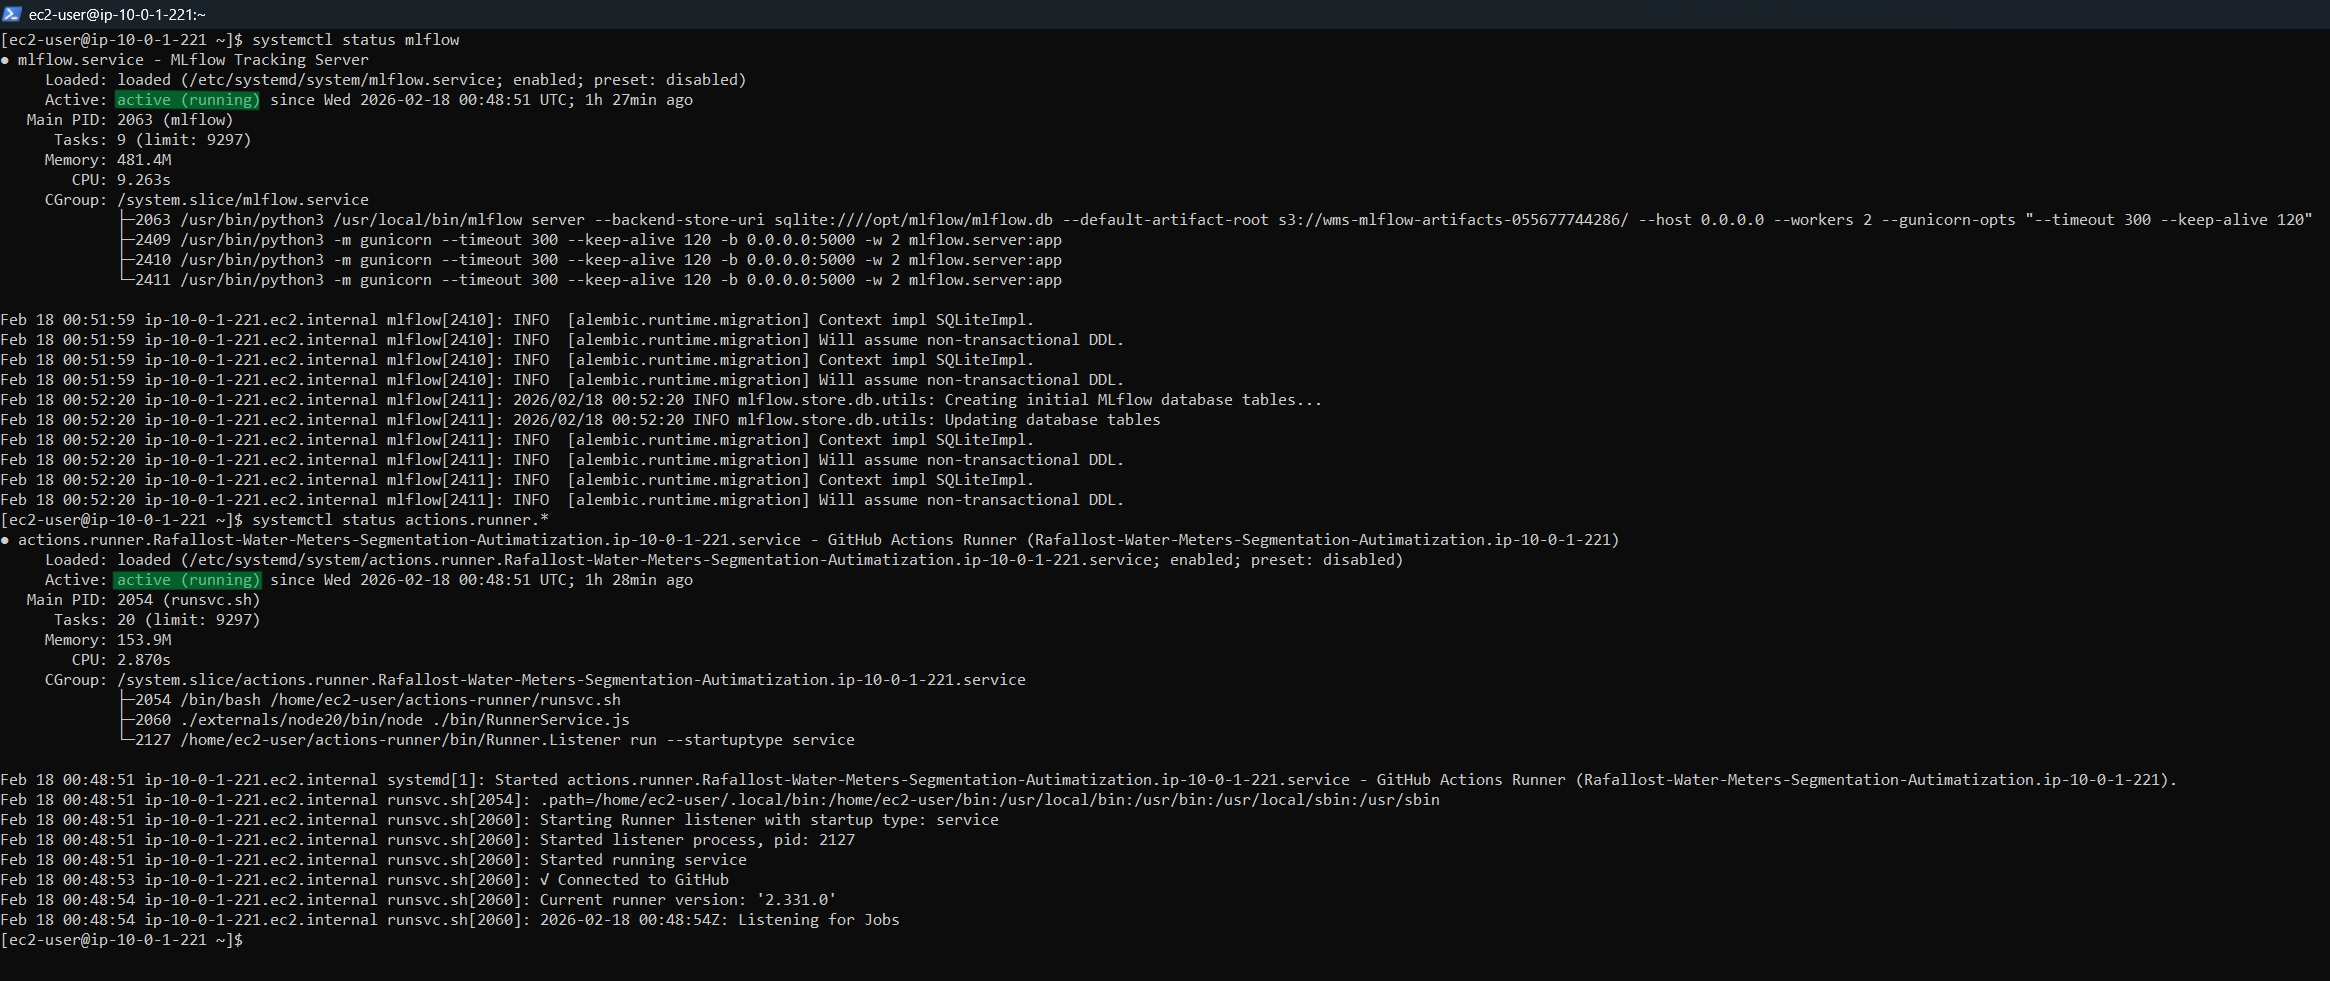
\includegraphics[width=\linewidth]{img/06_wdrozenie_systemu/systemctl_status.png}
  \caption{Stan usług \texttt{mlflow} i \texttt{actions.runner} w systemd --- obie usługi aktywne}
  \label{fig:systemctl-status}
\end{figure}

\begin{figure}[H]
 \centering
  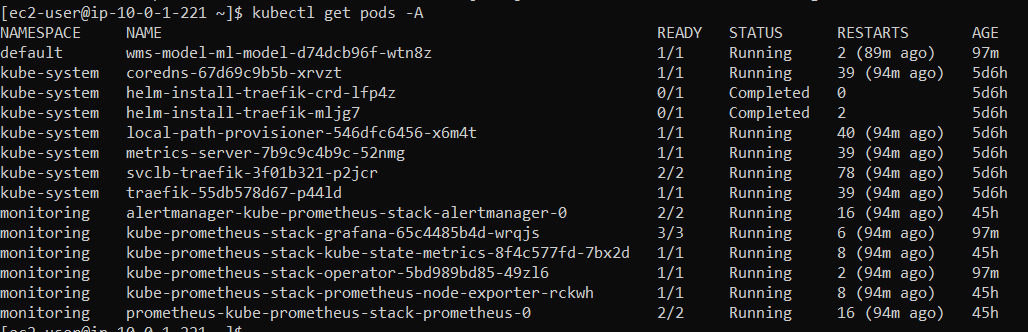
\includegraphics[width=\linewidth]{img/06_wdrozenie_systemu/kubectl_pods.png}
  \caption{Pody klastra k3s --- \texttt{kubectl get pods -A}. Widoczny pod API modelu oraz stos monitorowania.}
  \label{fig:kubectl-pods}
\end{figure}

Interfejs MLflow dostępny jest pod adresem \texttt{http://100.50.251.97:5000} (rys.~\ref{fig:mlflow-ui}).

\begin{figure}[H]
 \centering
 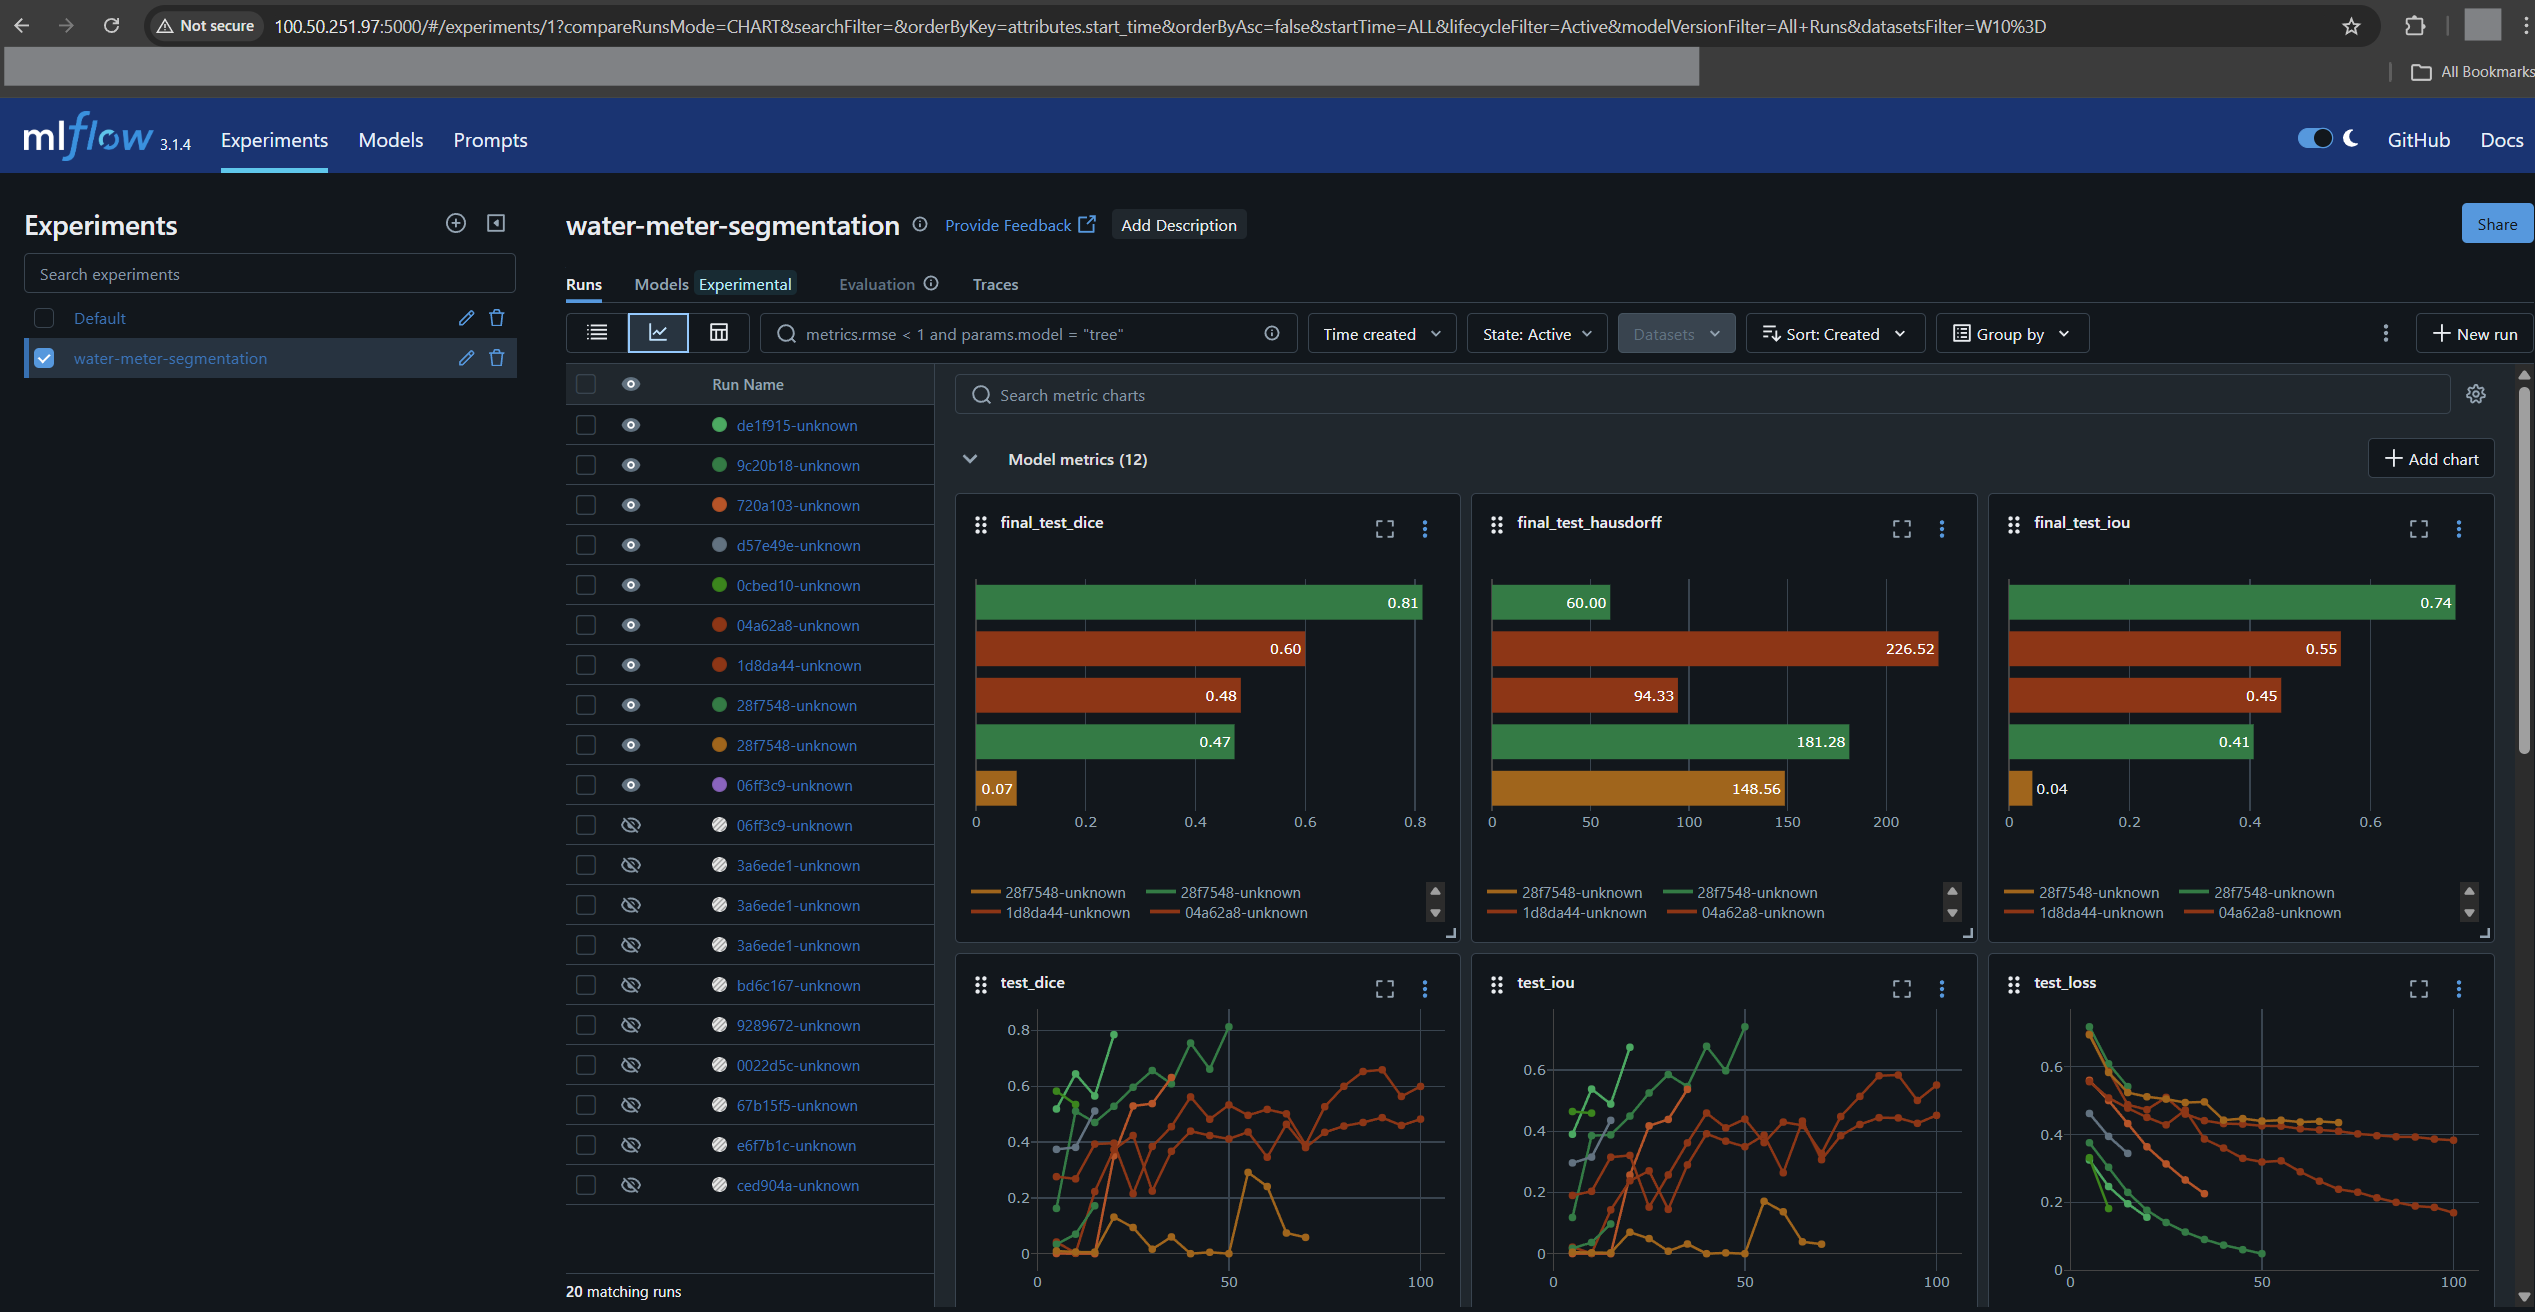
\includegraphics[width=\linewidth]{img/06_wdrozenie_systemu/mlflow_ui.png}
 \caption{Interfejs MLflow (\texttt{http://100.50.251.97:5000}) --- lista eksperymentów i przebiegów treningowych z metrykami}
 \label{fig:mlflow-ui}
\end{figure}

\subsection{Dostępne porty i usługi}
\label{subsec:porty}

Security Group Terraform otwiera wyłącznie porty niezbędne do działania systemu. Tabela~\ref{tab:ports} zestawia wszystkie dostępne punkty dostępu.

\begin{table}[H]
\centering
\caption{Porty dostępne na instancji EC2 \texttt{wms-k3s}}
\label{tab:ports}
\begin{tabular}{|c|l|l|}
\hline
\textbf{Port} & \textbf{Usługa} & \textbf{Przeznaczenie} \\
\hline
22   & SSH             & Zarządzanie instancją EC2 (tylko IP operatora) \\
\hline
5000 & MLflow          & Interfejs śledzenia eksperymentów i rejestr modeli \\
\hline
30080 & API modelu (NodePort) & Predykcja segmentacji --- endpoint \texttt{/predict} \\
\hline
30300 & Grafana (NodePort)    & Dashboard wizualizacji metryk \\
\hline
30900 & Prometheus (NodePort) & Interfejs zapytań i podgląd \textit{Targets} \\
\hline
\end{tabular}
\end{table}

Ruch przychodzący na porty 5000, 30080, 30300 i 30900 jest dozwolony z dowolnego adresu IP (\texttt{0.0.0.0/0}), ponieważ EC2 nie jest wyposażone w Load Balancer z certyfikatem TLS, a połączenia odbywają się po HTTP. Port SSH (22) jest ograniczony do konkretnego adresu IP operatora skonfigurowanego w \texttt{terraform.tfvars}. Konfigurację Security Group przedstawia rysunek~\ref{fig:security-group}.

\begin{figure}[H]
  \centering
  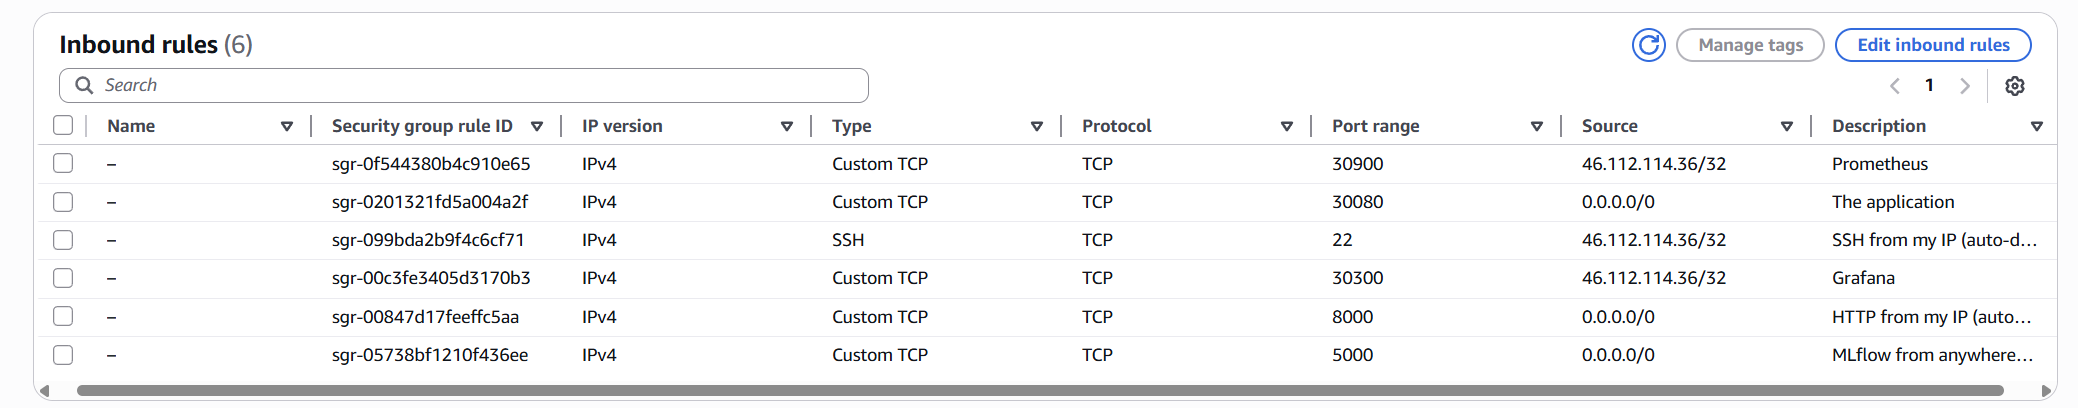
\includegraphics[width=\linewidth]{img/06_wdrozenie_systemu/security_groups.png}
  \caption{Security Group instancji EC2 --- reguły ruchu przychodzącego z otwartymi portami usług}
  \label{fig:security-group}
\end{figure}

\subsection{Konfiguracja Helm}

W projekcie Helm \cite{helm_docs} wykorzystywany jest dwojako: do wdrożenia własnego charta API modelu oraz do konfiguracji zewnętrznego stosu monitorowania.

\textbf{Chart API modelu.} Katalog \texttt{devops/helm/ml-model/} zawiera własny chart Kubernetes dla serwera API. Zamiast zarządzać oddzielnymi plikami manifestów, całą aplikację opisuje jeden zestaw szablonów YAML sparametryzowanych zmiennymi. Bez Helm każda aktualizacja wymagałaby ręcznej edycji kilku plików i kolejnych wywołań \texttt{kubectl apply}. Helm sprowadza to do jednej komendy:

\begin{verbatim}
helm upgrade --install wms-model devops/helm/ml-model/ \
  -f infrastructure/helm-values.yaml \
  --namespace default --create-namespace
\end{verbatim}

Komenda ta działa zarówno przy pierwszym wdrożeniu (\textit{install}) jak i przy aktualizacji (\textit{upgrade}); Helm sam sprawdza czy release już istnieje. Helm zachowuje historię wdrożeń (\texttt{helm history wms-model}), co umożliwia szybki rollback do poprzedniej wersji.

Struktura charta:

\begin{verbatim}
devops/helm/ml-model/
+-- Chart.yaml              <- metadane (nazwa, wersja charta)
+-- values.yaml             <- wartosci domyslne (NodePort 30080, limity RAM/CPU)
\-- templates/
    +-- _helpers.tpl        <- funkcje pomocnicze Helm
    +-- deployment.yaml     <- zasob Deployment
    +-- service.yaml        <- zasob Service (NodePort 30080)
    \-- servicemonitor.yaml <- ServiceMonitor dla Prometheus
\end{verbatim}

Szablony korzystają ze składni Go Templates i odwołują się do wartości przez \texttt{.Values.*}. Plik \texttt{infrastructure/helm-values.yaml} nadpisuje wartości domyślne charta dla konkretnego wdrożenia. Najważniejsze fragmenty:

\begin{verbatim}
image:
  repository: "055677744286.dkr.ecr.us-east-1.amazonaws.com/wms-model"
  pullPolicy: Always
  tag: "latest"

imagePullSecrets:
  - name: ecr-secret    # dane do logowania do ECR

env:
  - name: MLFLOW_TRACKING_URI
    value: "http://localhost:5000"  # MLflow na hoscie EC2 (hostNetwork)
  - name: MODEL_VERSION
    value: "production"

resources:
  limits:
    memory: "1Gi"
    cpu: "500m"
  requests:
    memory: "512Mi"
    cpu: "100m"
\end{verbatim}

Warto zwrócić uwagę na \texttt{MLFLOW\_TRACKING\_URI: localhost:5000}; kontener korzysta z \texttt{hostNetwork: true}, co pozwala mu odwoływać się do MLflow działającego bezpośrednio na maszynie EC2, bez konieczności dodatkowej usługi Kubernetes. Przy każdym wdrożeniu GitHub Actions podaje aktualny hash commita jako \texttt{--set image.tag=\$\{COMMIT\_SHA\}}, co zapewnia jednoznaczną identyfikację wersji obrazu.

Postęp wdrożenia API można śledzić w czasie rzeczywistym poleceniem:
\begin{verbatim}
kubectl rollout status deployment/wms-model-ml-model --watch
\end{verbatim}

Po wdrożeniu API jest dostępne pod adresem \texttt{http://100.50.251.97:30080}.

\begin{figure}[H]
 \centering
 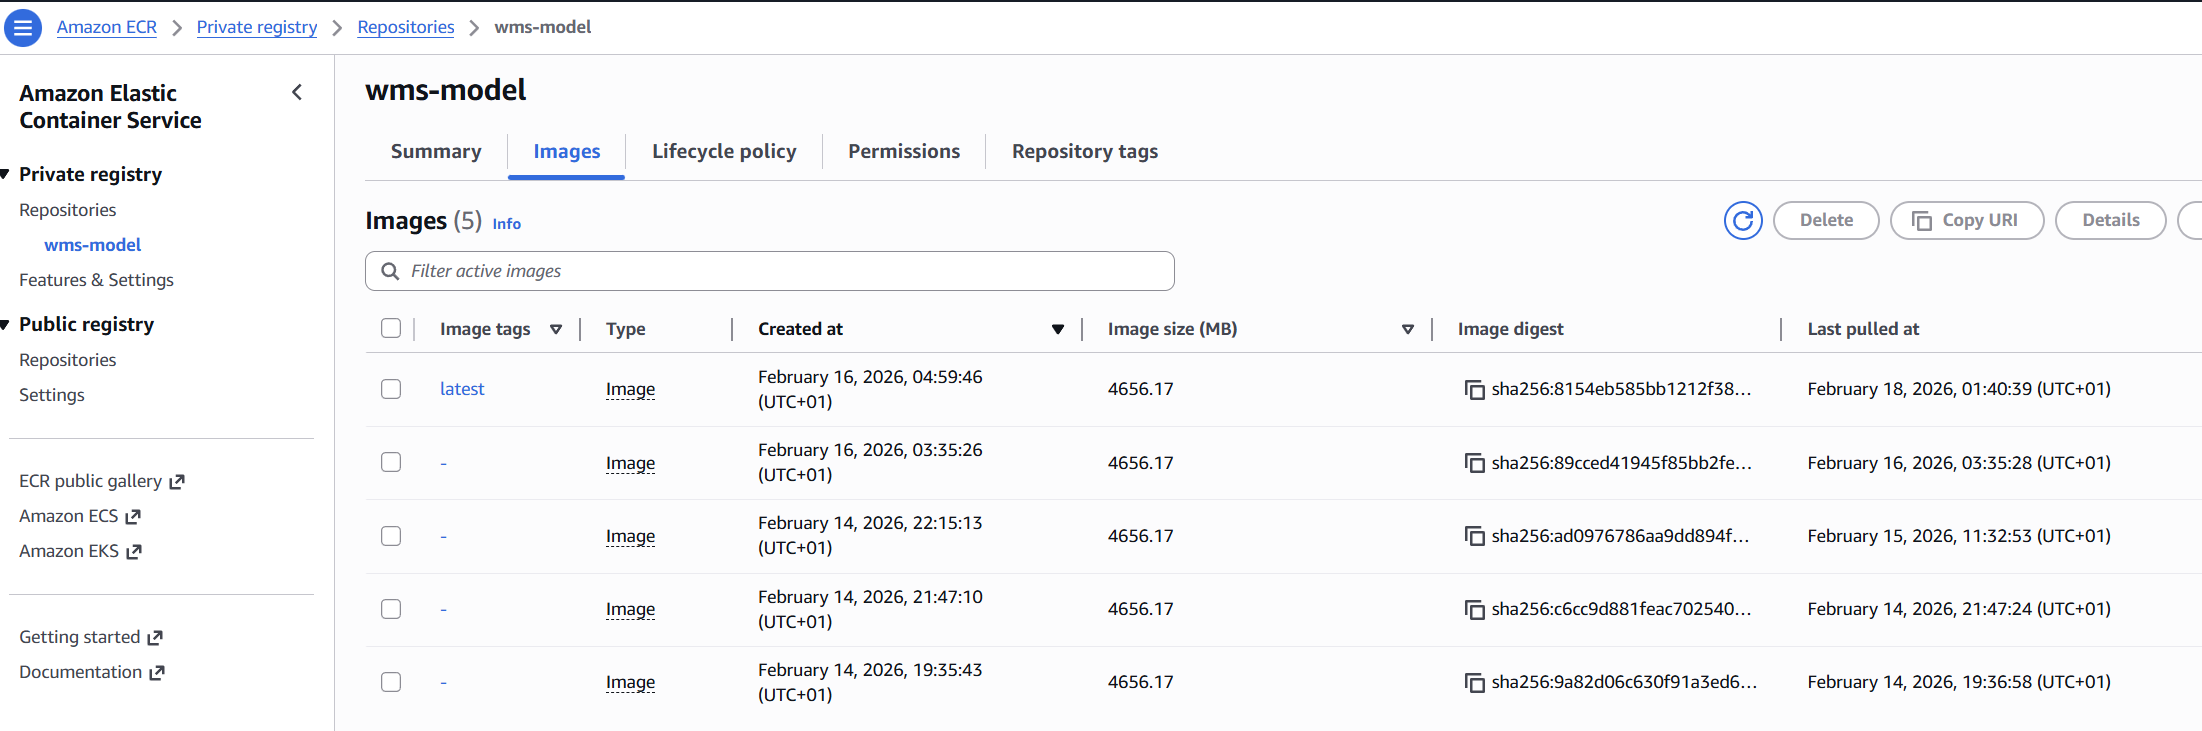
\includegraphics[width=0.9\linewidth]{img/06_wdrozenie_systemu/ecr_repository.png}
 \caption{Repozytorium \texttt{wms-model} w Amazon ECR z obrazami oznaczonymi hashiem commita}
 \label{fig:ecr-repo}
\end{figure}

Dostępne endpointy API to \texttt{/health} (status usługi), \texttt{/predict} (predykcja segmentacji) i \texttt{/metrics} (metryki Prometheus). Odpowiedź endpointu \texttt{/health} przedstawia rysunek~\ref{fig:api-health}, a pełną listę eksponowanych metryk prezentuje rysunek~\ref{fig:metrics}.

\begin{figure}[H]
  \centering
  \begin{subfigure}[t]{0.48\linewidth}
    \centering
    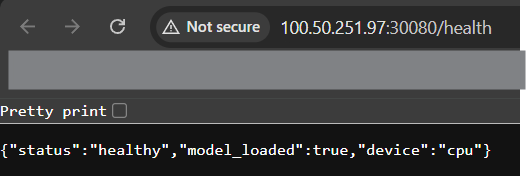
\includegraphics[width=\linewidth]{img/06_wdrozenie_systemu/api_health.png}
    \caption{Odpowiedź endpointu \texttt{/health} wdrożonego API modelu}
    \label{fig:api-health}
  \end{subfigure}
  \hfill
  \begin{subfigure}[t]{0.48\linewidth}
    \centering
    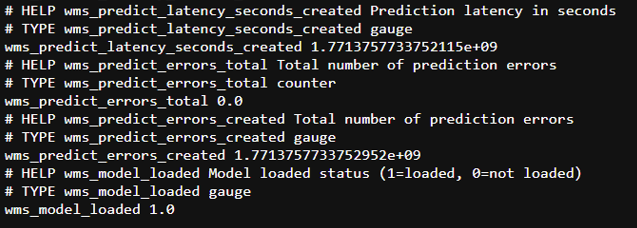
\includegraphics[width=\linewidth]{img/06_wdrozenie_systemu/metrics_short.png}
    \caption{Metryki Prometheus eksponowane pod adresem \texttt{/metrics}: liczba predykcji, czasy odpowiedzi i błędy}
    \label{fig:metrics}
  \end{subfigure}
  \caption{Endpointy diagnostyczne API modelu}
  \label{fig:api-endpoints}
\end{figure}

\subsection{Stos monitorowania}

Monitoring oparty na Prometheus \cite{prometheus_docs} i Grafana wdrażany jest jako oddzielny stos na tym samym klastrze k3s. Składa się z trzech komponentów:

\begin{itemize}
  \item \textbf{Prometheus} --- zbiera metryki z endpointu \texttt{/metrics} API modelu co 15 sekund; konfiguracja scraping w \texttt{prometheus.yml},
  \item \textbf{Grafana} --- wizualizuje metryki na predefiniowanych dashboardach; dostępna na porcie NodePort 30300,
  \item \textbf{kube-state-metrics} --- dostarcza metryki Kubernetes (stan podów, zużycie zasobów węzła).
\end{itemize}

\begin{sloppypar}
API modelu eksponuje metryki w formacie Prometheus przy użyciu biblioteki \texttt{prometheus\_client}. Śledzone metryki to:
\end{sloppypar}
\begin{itemize}
  \item \texttt{wms\_predictions\_total} --- łączna liczba żądań predykcji (Counter),
  \item \texttt{wms\_predict\_latency\_seconds} --- histogram czasów odpowiedzi,
  \item \texttt{wms\_predict\_errors\_total} --- liczba błędów (Counter),
  \item \texttt{wms\_model\_loaded} --- czy model jest załadowany (Gauge, wartość 0 lub 1).
\end{itemize}

Działanie stosu monitorowania ilustruje dashboard Grafana (rys.~\ref{fig:grafana-dashboard}) oraz widok Targets w Prometheus (rys.~\ref{fig:prometheus-targets}).

\begin{figure}[H]
 \centering
 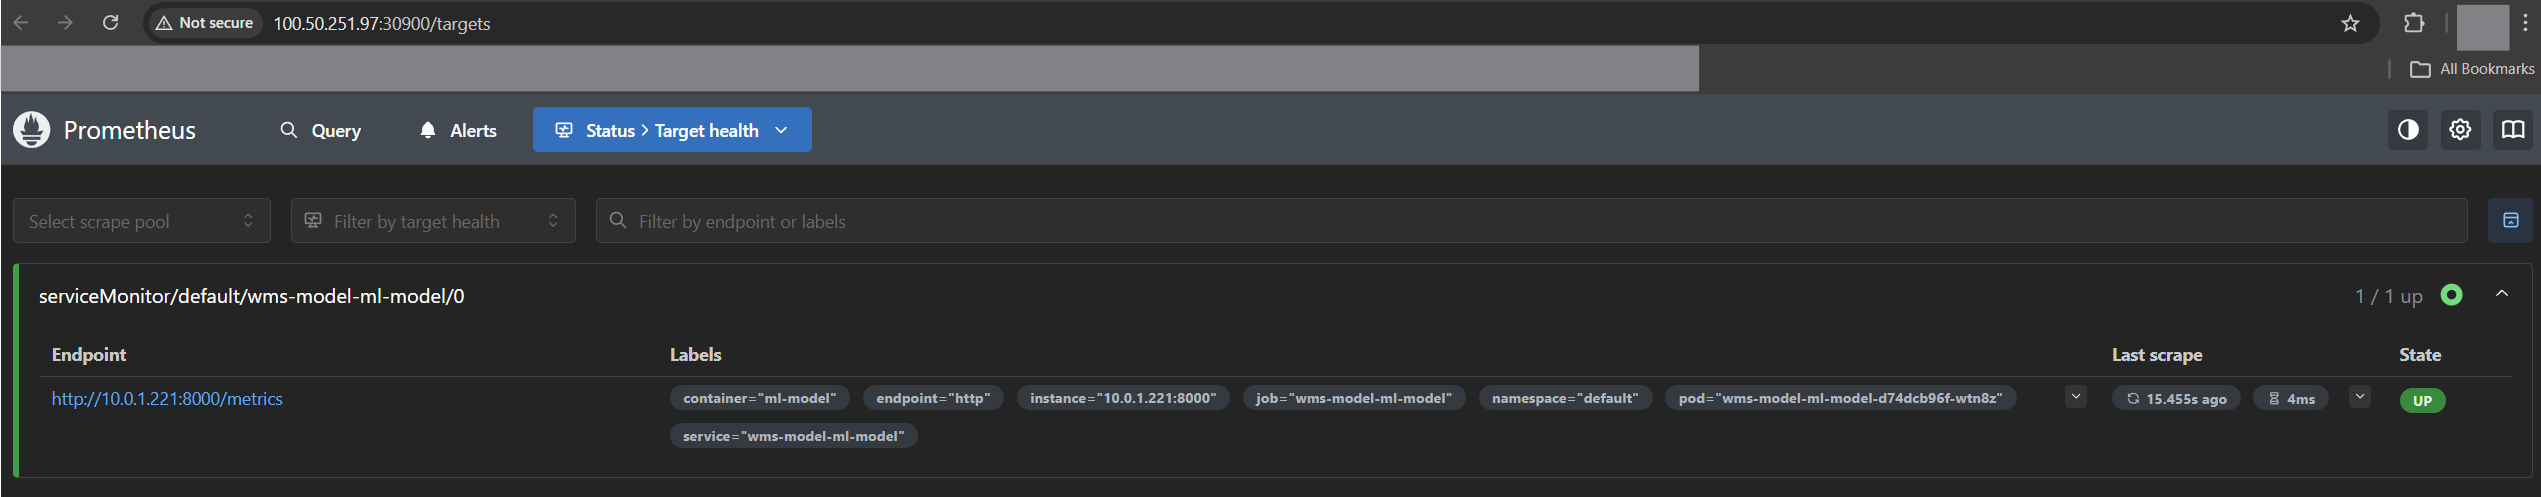
\includegraphics[width=\linewidth]{img/06_wdrozenie_systemu/prometheus_targets.png}
 \caption{Strona \textit{Targets} w Prometheus (\texttt{:30900}) --- endpoint \texttt{/metrics} API w stanie \texttt{UP}}
 \label{fig:prometheus-targets}
\end{figure}

\begin{figure}[H]
 \centering
 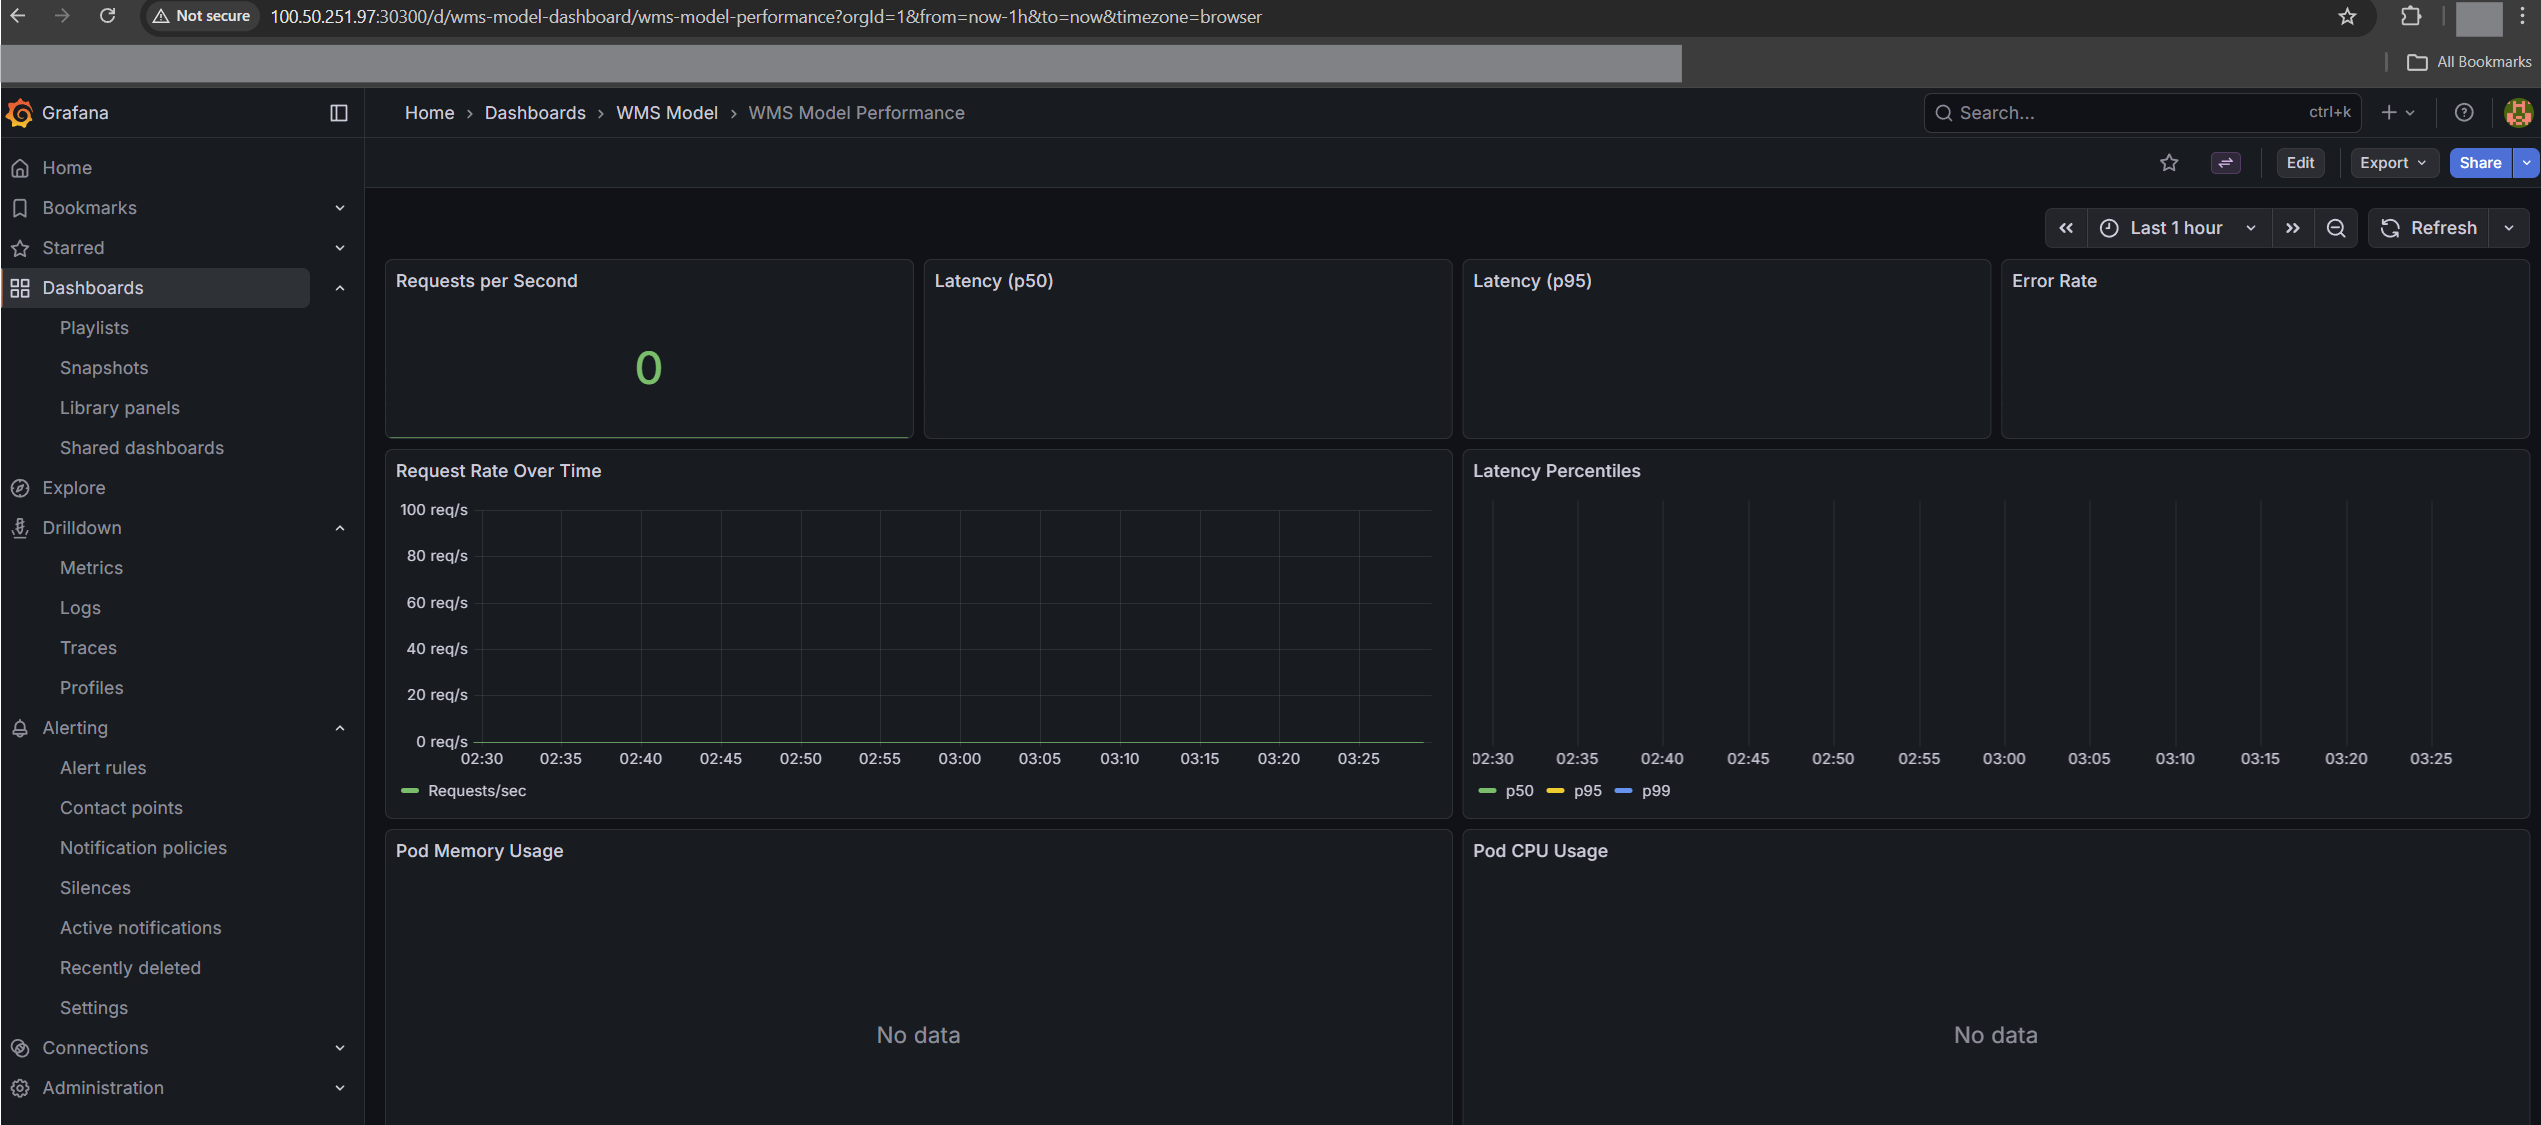
\includegraphics[width=\linewidth]{img/06_wdrozenie_systemu/grafana_dashboard.png}
 \caption{Dashboard Grafana (\texttt{http://100.50.251.97:30300}) --- metryki działającego API modelu}
 \label{fig:grafana-dashboard}
\end{figure}

\subsection{Workflow użytkownika}

\subsubsection{Scenariusz 1: Wdrożenie przez automatyczny pipeline}

Jak opisano w rozdziale~\ref{sec:Pipeline_CICD}, dostarczenie nowych danych treningowych przez \texttt{git push} wyzwala pełny pipeline. Jeśli wytrenowany model przeszedł bramkę jakości, pipeline automatycznie wdraża go na klaster k3s przez \texttt{deploy-model.yaml}, a następnie zatrzymuje instancję EC2. Po zakończeniu pipeline'u aplikacja jest zainstalowana na klastrze i gotowa do działania. Aby skorzystać z API, wystarczy uruchomić instancję EC2 za pomocą workflow \textit{Manual EC2 Control} (zakładka \textit{Actions} w GitHub, akcja \textit{start}). Po uruchomieniu workflow wyświetla adres IP w podsumowaniu, a endpoint \texttt{/predict} jest natychmiast dostępny.

Należy zaznaczyć, że wdrożenie następuje tylko gdy model poprawił metryki. Jeśli trening nie przeszedł bramki jakości, klaster k3s nadal serwuje poprzednią wersję. Do kontrolowanego wdrożenia niezależnego od treningu służy Scenariusz~2.

\subsubsection{Scenariusz 2: Ręczne wdrożenie i korzystanie z API (zalecany)}

Jest to zalecany sposób korzystania z systemu dla operatora chcącego uruchomić lub zaktualizować działające API. Cały proces odbywa się przez interfejs GitHub Actions i nie wymaga żadnych lokalnych poświadczeń AWS.

\textbf{Krok 1: Wdrożenie modelu.} W zakładce \textit{Actions} należy uruchomić workflow \textit{Release \& Deploy} (\texttt{release-deploy.yaml}) klikając \textit{Run workflow}. Workflow automatycznie uruchamia instancję EC2, buduje obraz Docker, wypycha go do ECR, pobiera najnowszy model ze stadium Production z MLflow, aktualizuje klaster k3s przez Helm, a po weryfikacji zatrzymuje EC2.

\textbf{Krok 2: Uruchomienie instancji do predykcji.} Po wdrożeniu model jest zainstalowany na klastrze, ale EC2 jest zatrzymany w celu oszczędności. Aby wysyłać zapytania do API, należy uruchomić instancję workflow \textit{Manual EC2 Control} z akcją \textit{start}. Workflow wyświetla aktualne IP i URL MLflow w podsumowaniu uruchomienia. API jest dostępne pod adresem \texttt{http://100.50.251.97:30080/}.

\begin{figure}[H]
  \centering
  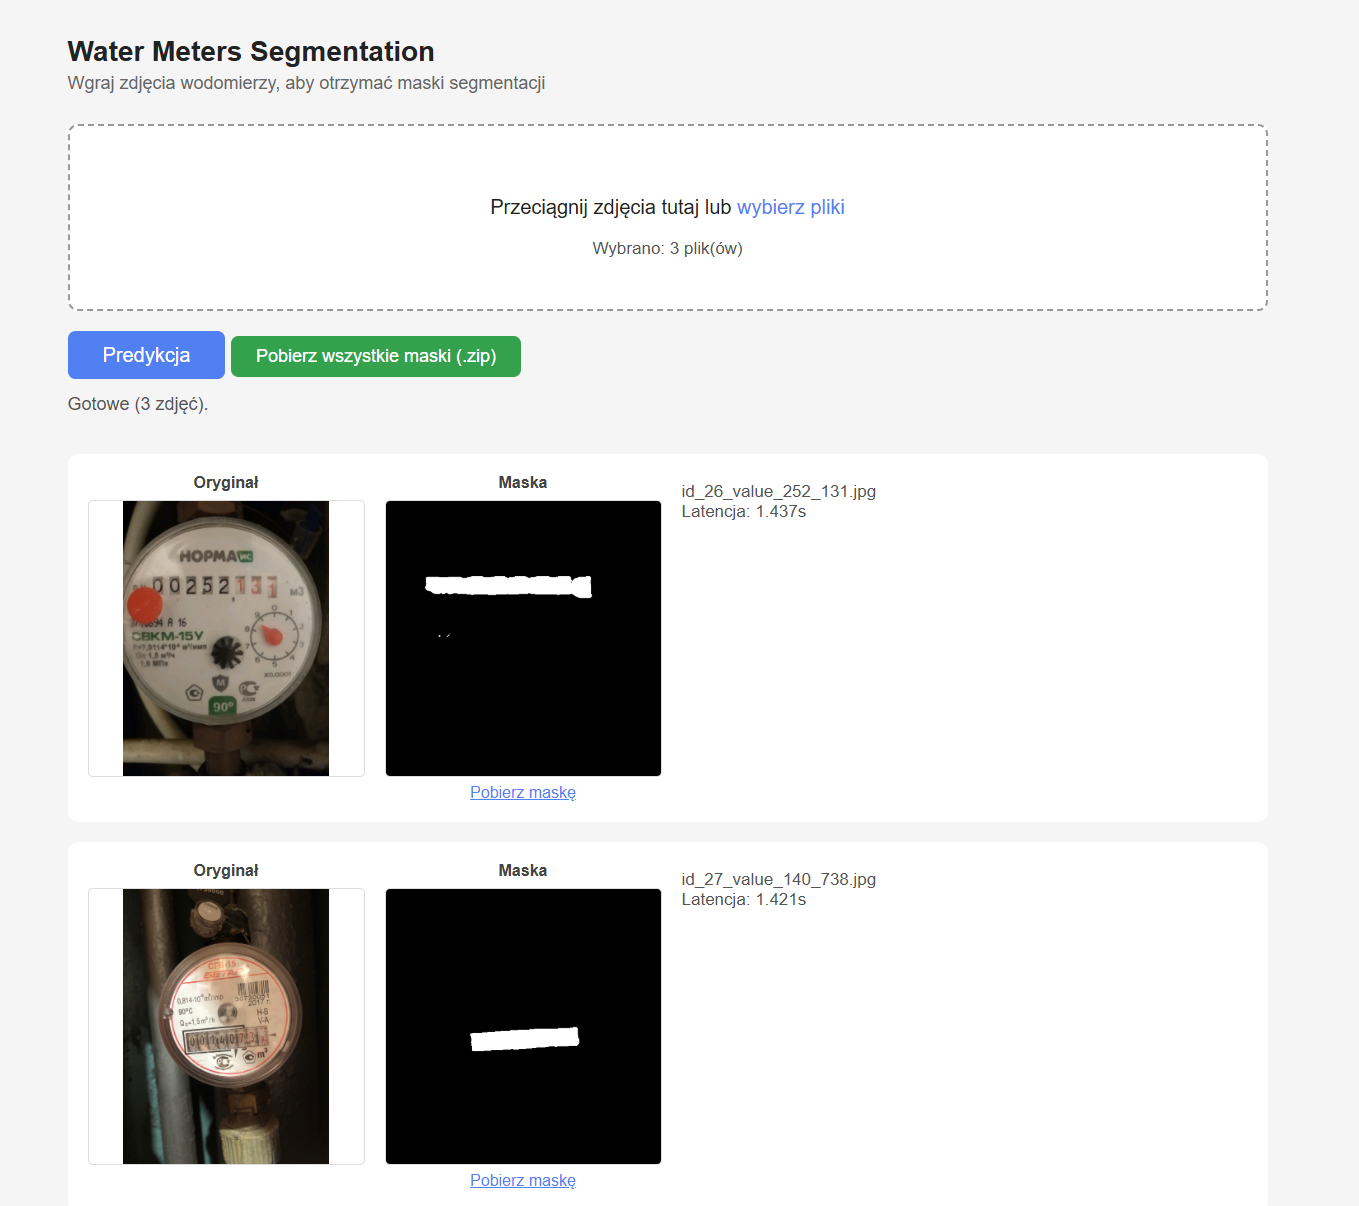
\includegraphics[width=\linewidth]{img/06_wdrozenie_systemu/deployed_app.png}
  \caption{Działający interfejs webowy API modelu: segmentacja trzech zdjęć wodomierzy z wygenerowanymi maskami i zmierzoną latencją predykcji}
  \label{fig:deployed-app}
\end{figure}

Po zakończeniu pracy należy ponownie uruchomić \textit{Manual EC2 Control} z akcją \textit{stop}, aby nie generować zbędnych kosztów.

\subsubsection{Scenariusz 3: Lokalna predykcja (wyłącznie dla deweloperów)}

Predykcję można uruchomić lokalnie bez infrastruktury chmurowej. Opcja ta wymaga jednak spełnienia warunków niedostępnych dla typowego użytkownika końcowego.

Wymagania wstępne:
\begin{itemize}
  \item działająca instancja EC2 z MLflow (model musi być zarejestrowany w stadium Production),
  \item lokalne poświadczenia AWS skonfigurowane w \texttt{\textasciitilde/.aws/credentials}: \texttt{AWS\_ACCESS\_KEY\_ID}, \texttt{AWS\_SECRET\_ACCESS\_KEY}, \texttt{AWS\_SESSION\_TOKEN},
  \item Python z zależnościami projektu zainstalowanymi lokalnie.
\end{itemize}

Przy spełnieniu powyższych warunków predykcja przebiega następująco:
\begin{enumerate}
  \item Pobranie modelu Production z MLflow na dysk lokalny:
        \begin{lstlisting}[numbers=none,frame=none,backgroundcolor=\color{white},basicstyle=\ttfamily\small,xleftmargin=0pt]
python WMS/scripts/sync_model_aws.py
\end{lstlisting}
  \item Umieszczenie obrazów do segmentacji w \texttt{WMS/data/predict/input/}.
  \item Uruchomienie predykcji: \texttt{python WMS/src/predicts.py}
  \item Wyniki zapisywane są w \texttt{WMS/data/predict/output/}.
\end{enumerate}

Poświadczenia AWS w środowisku AWS Academy są tymczasowe (ważność 4~godziny) i wymagają ręcznego odnawiania przy każdej sesji laboratoryjnej. Z tego powodu opcja lokalnej predykcji jest praktycznie dostępna wyłącznie dla operatora posiadającego bezpośredni dostęp do konta AWS, a nie dla użytkownika końcowego.

Opisane scenariusze pokrywają wszystkie typowe przypadki interakcji z systemem.

\subsection{Dostępne operacje zarządzania wdrożeniem}

System udostępnia cztery workflow GitHub Actions do zarządzania infrastrukturą i wdrożeniami. Tabela~\ref{tab:workflows} zestawia je wraz z wyzwalaczami i przeznaczeniem.

\begin{table}[H]
\centering
\caption{Workflow GitHub Actions dostępne w systemie}
\label{tab:workflows}
\begin{tabular}{|p{4.2cm}|p{3.2cm}|p{6.5cm}|}
\hline
\textbf{Workflow} & \textbf{Wyzwalacz} & \textbf{Przeznaczenie} \\
\hline
\texttt{training-data-pipeline} & Push do \texttt{data/*}, \texttt{workflow\_dispatch} & Pełny pipeline: pobieranie danych z S3, walidacja, trening, bramka jakości. Jeśli model poprawił metryki: wdrożenie na k3s i scalenie PR. EC2 uruchamiany i zatrzymywany automatycznie. \\
\hline
\texttt{release-deploy} & Push do \texttt{main} (zmiany kodu/Docker/Helm), \texttt{workflow\_dispatch} & Wdrożenie modelu na klaster k3s bez treningu: build Docker, push do ECR, aktualizacja Helm. Używany przy zmianach kodu serwowania lub jako ręczne ponowne wdrożenie. EC2 uruchamiany i zatrzymywany automatycznie. \\
\hline
\texttt{ec2-manual-control} & Tylko \texttt{workflow\_dispatch} & Ręczne uruchomienie lub zatrzymanie instancji EC2. Po starcie wyświetla aktualne IP i URL MLflow w podsumowaniu. Używany gdy potrzebny jest dostęp do API lub interfejsu MLflow. \\
\hline
\texttt{deploy-model} & Reużywalny (\texttt{workflow\_call}), \texttt{workflow\_dispatch} & Właściwy krok wdrożenia wywoływany przez \texttt{training-data-pipeline} i \texttt{release-deploy}. Można też uruchomić samodzielnie. Działa na self-hosted runnerze EC2, uwierzytelniając się przez rolę IAM instancji. \\
\hline
\end{tabular}
\end{table}

Żaden z powyższych workflow nie wymaga lokalnych poświadczeń AWS na komputerze operatora. Workflow uruchamiane na runnerze \texttt{ubuntu-latest} (start/stop EC2) korzystają z sekretów repozytorium GitHub, natomiast \texttt{deploy-model} działa na self-hosted runnerze EC2 i uwierzytelnia się przez rolę IAM przypisaną do instancji.

